\chapter{Background}
\index{Background%
@\emph{Background}}%
\label{ch:background}

When the Web was first created by Tim Berners-Lee\index{Berners-Lee, Tim} in 1989, web pages were largely envisioned as static \textit{documents} with a single author or a small group of coordinating authors. 
The idea of composing a complex web application out of basic components like snapping together Lego blocks seemed like a distant dream at best.
Until recently, web authors were limited to using the predefined HTML layout elements or `tags' that were listed in the W3C standard and understood by browser programs, such as \tcode{<title>} and \tcode{<video>}. 
Creating your own \textit{sui generis} HTML elements with unique behaviors seemed beyond the capabilities of the web browsers of the day like Mosaic\index{Mosaic}
and Netscape Navigator\index{Netscape Navigator}.

As of early 2015, modern web apps are typically written with a JavaScript\index{JavaScript} framework that provides a cohesive set of structures, design patterns and practices designed to facilitate composing web applications 
--- large or small --- 
from a number of sub-components.
Angular\index{Angular}, Meteor\index{Meteor}, and Backbone\index{Backbone} are three such frameworks~\cite{dickey2014}.
The difference between a `framework'\index{Framework} and a library is somewhat arbitrary, but typically frameworks are more comprehensive than narrowly focused utility libraries.
Yet all frameworks must exist within the confines of the programming model provided by the browser and the Document Object Model (DOM)\index{DOM}. 
In this model, the entire web page or app belongs to a single `document', constituent parts are not encapsulated\index{encapsulation} or isolated from each other, and authors are limited to working with the predefined HTML tags.
These issues make it difficult to create and share generic, reusable \textit{web components} 
--- in the abstract sense --- 
among different users who may not use the same frameworks or follow the same set of assumptions and conventions.

\section{Current challenges in web authoring}
In object oriented programming, encapsulation\index{encapsulation} is typically defined as a 
``language mechanism for restricting access to some of the object's components''
~\cite[p. 522]{mitchell2003}.
The point of encapsulation is providing an \textit{abstraction} that consumers of the functionality can rely on without knowing the internals. 
The goals of encapsulation and abstraction include:
\begin{quote}
Identifying the interface of a data structure~\dots~providing \textit{information hiding} by separating implementation decisions from parts of the program that use the data 
structure~\dots~and allowing the data structure to be used in many different ways by many different components~\cite[p. 243]{mitchell2003}.
\end{quote}

Although techniques of abstraction\index{abstraction} and encapsulation\index{encapsulation} have been widespread in object oriented programming for decades,
the fundamental web client programming model has not allowed for significant encapsulation of things like the DOM structure and CSS style rules~\cite{ihrig2012}.

To illustrate how these problems affect the ability of authors to share and reuse code, let's look at an example from the popular Twitter\index{Twitter} Bootstrap\index{Bootstrap} library~\cite{bootstrapcontributors2015}.
Twitter Bootstrap is a collection of Cascading Style Sheet (CSS)\index{CSS} rules and JavaScript\index{JavaScript} widgets or components designed to allow web authors to quickly `bootstrap' an attractive, consistent look-and-feel onto a web page.
Bootstrap provides pre-styled user interface\index{user interface (UI)} (UI) widgets such as menus, buttons, panels, dropdown selectors, alerts, dialogs, and so on, to be used as building blocks to construct web sites or application user interfaces.
Because Bootstrap must work within the confines of the DOM\index{DOM} and the HTML5\index{HTML!HTML5} standard, this necessarily exposes a great deal of Bootstrap's internals to its users.
For example, to add a Bootstrap site navigation bar to your page, you must essentially copy and paste a large block of HTML\index{HTML} and then customize it to your needs as shown in Figure~\ref{f:twbs1}.

\begin{figure}[htb]
\centering
 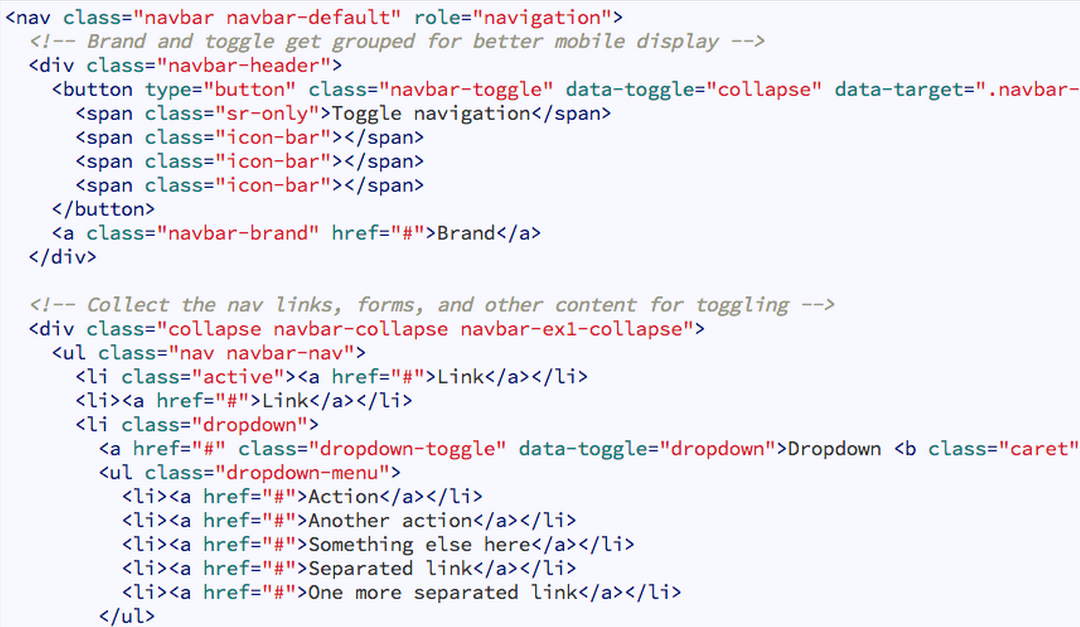
\includegraphics[width=6in]{images/bootstrap_navbar_html.png}
\caption{Partial example of Twitter\index{Twitter} Bootstrap\index{Bootstrap} navigation bar HTML.}
\label{f:twbs1}
\end{figure}


This forces Bootstrap's\index{Bootstrap} users to tightly couple the layout of their page with the internal structure required by Bootstrap's navigation bar widget. 
This coupling hinders a significant refactoring\index{refactoring} of the navigation widget's internal structure (HTML\index{HTML} layout) because that would require the large community of developers to update their applications accordingly.
In addition, because CSS\index{CSS} rules normally apply across the entire page, the authors of Bootstrap must carefully select the scope and nomenclature of all rules to ensure no unintended side-effects~\cite{walton2014}. 
Even then, conflicts are inevitable when the entire page is treated as a single sandbox and you combine components from many different vendors. 

What if instead one could create and share a reusable chunk of functionality --- a web component -- that hid all of these tedious structural details and encapsulated its private, internal state? 
What if web authors could create their \textit{own} HTML elements?  
Using Bootstrap's navigation bar could be as easy as replacing the code in figure~\ref{f:twbs1} with a custom element like the one in the following example:

% 
%\begin{figure}[htb]
%\centering
% 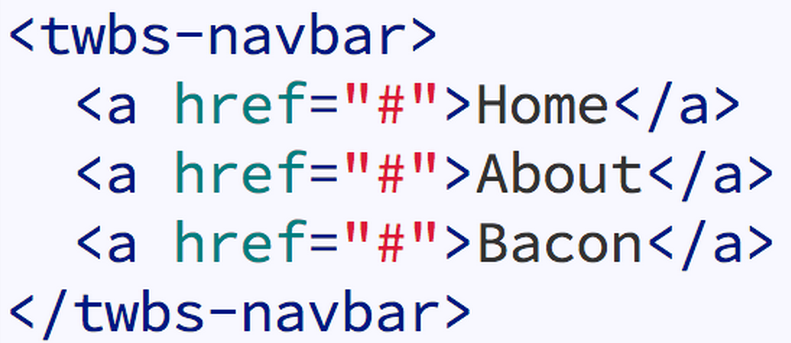
\includegraphics[width=3.5in]{images/bootstrap_navbar_wc.png}
%\caption{Hypothetical Bootstrap nav bar custom element.}
%\label{f:twbs2}
%\end{figure}

\begin{lstlisting}[language=HTML5,numbers=none,caption=
{Hypothetical Bootstrap nav bar custom element.},label=l:twbs2,captionpos=below]
 <twbs-navbar>
   <a href="#">Home</a>
   <a href="#">About</a>
   <a href="#">Sign In</a>
 </twbs-navbar>
\end{lstlisting}

\subsection{Abstraction, encapsulation and composition}

The Web Components working group, consisting of software engineers\index{software engineering} from several major browser vendors, 
looked at this situation and found that, in practice, browsers already had a suitable model for encapsulating components that hide complexity behind well-defined interfaces.
That model was that one used internally by browsers to implement the newer 
HTML5\index{HTML!HTML5} tags 
like the \textbf{\tcode{<video>}} element.\index{<video>} 
The \tcode{<video>} element presents a simple interface (API) to HTML authors that hides the complexities of playing high definition video.
Internally, however, browsers implement \tcode{<video>} with a `shadow' or hidden document inside the object that contains the internal state~\cite{kitamura2014}. 
For example, an author can write:
\begin{lstlisting}[language=HTML5,numbers=none]
	<video loop src=...> </video>
\end{lstlisting}
to cause the video to loop repeatedly.

This shadow\index{Shadow DOM} Document Object Model (DOM)\index{DOM} inside the 
\tcode{<video>}\index{<video>} tag creates the user interface (UI) needed to control video playback such as the volume controls, the timeline bar, and the pause and play buttons.
These inner playback controls are themselves built out of HTML, CSS\index{CSS} and JS but these details are not exposed to web authors who simply place a \tcode{<video>} element on their page. 
Figure~\ref{f:html5video} illustrates how this works. It shows the shadow (internal) DOM of a \tcode{<video>} element on a page with the Play button \tcode{<div>} highlighted.

\begin{figure}[htb]
\centering
 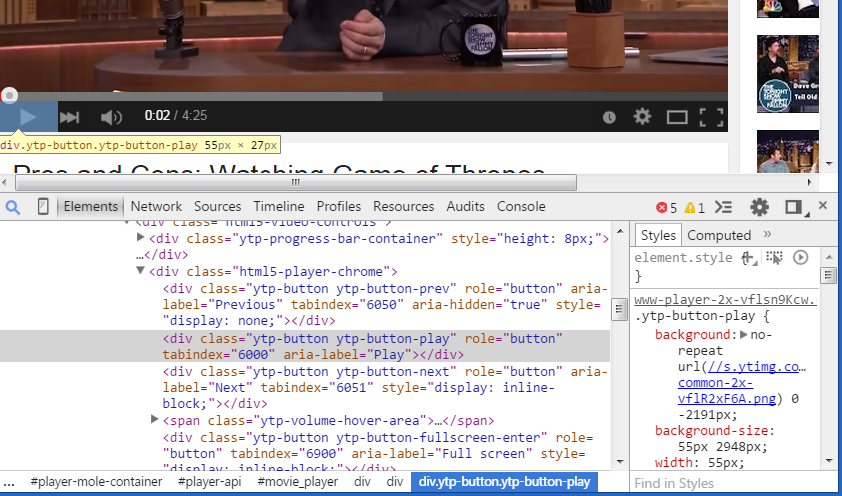
\includegraphics[width=5.5in]{images/html5_video_control.png}
\caption{Opera's shadow DOM for \tcode{<video>}\index{<video>} highlighting the Play button}
\label{f:html5video}
\end{figure}

At the bottom of Figure~\ref{f:html5video} a small \tcode{\#player-api} tag is visible in the DOM path.
This is an example of the container inside \tcode{<video>}\index{<video>} using the abstraction of a \tcode{\#player-api} to encapsulate the details of actually controlling playback within the context of the overall \tcode{<video>} interface.

This example illustrates three component design principles that are widely followed in other areas of software engineering\index{software engineering}~\cite{fowler2012}:
\begin{itemize}
\item Create layers of \textbf{abstraction}\index{abstraction} to represent `public' details that are relevant to the surrounding code or environment.
\item Use \textbf{encapsulation}\index{encapsulation} and well defined interfaces to protect private state, hide implementation complexity, and leave implementors free to refactor internals.
\item Prefer \textbf{composition}\index{composition} or \textit{has-a} relationships over inheritance or \textit{is-a} relationships when building modules to reduce coupling and simplify interface refactoring\index{refactoring}.
\end{itemize}

Composition helps reduce coupling or structural between modules by forcing them to interact using only public interfaces.
In the case of the interface for \tcode{<video>}, it's composed of simple block elements and scoped CSS\index{CSS} roles and the Volume and Play controls aren't particularly special objects, just \tcode{<divs>} with CSS rules and click handlers.

The solution, therefore, to these coupling problems in web authoring is to expose these internal brower APIs for creating elements in a safe and portable fashion. 
This will allow web authors to create their own rich custom elements using standard portable APIs, encapsulate their internals, and enable easier sharing, composition and integration.
The question remains, which specific browser internals must be exposed and standardized in order to support Web Components?

\section{Web Components}

Web Components consists of two main technologies and two supporting features. 
Custom HTML Elements\index{Custom Elements} and Shadow DOM\index{Shadow DOM} are the two key players while HTML Imports\index{HTML!Imports} and Templates\index{HTML!Templates} support these features. 
One of the central goals of the Web Components\index{Web Components} initiative is to maintain interoperability across different browsers and frameworks, 
so that modules which adhere to the Web Components standard can provide a consistent experience no matter what framework the developer chooses or which browser the user selects.
For example, an important benefit of Custom Elements is that they \textit{are} standard HTML elements; they live in the DOM\index{DOM} and can be accessed by the usual DOM methods and the majority of standard HTML/JS development tools~\cite{penades2015}.
They also behave somewhat like objects in traditional object oriented programming (OOP) in that 
they have \textit{methods} and hidden internal \textit{state} (data).

\subsection{Custom HTML elements}
Never before have web authors been able to define their own custom HTML elements\index{Custom Elements} that were not found in the official list.
Actually, many authors and web frameworks have been doing exactly that for years, primarily for internal purposes where the custom elements are pre\-processed and compiled down to standard HTML.
The custom elements would not get sent to the end user's browser because it would not know what to do with them.
In addition, the DOM\index{DOM} has long supported creating custom-named elements, but it was not possible to do much interesting with them because they were treated like an ordinary 
\tcode{<span>}\index{<span>} element~\cite{w3ccontributors2015-b}.
However, the possibility now exists to create custom elements in a standard way that will work consistently across browsers with the W3C Custom Element\index{Custom Elements}
specification~\cite{w3ccontributors2015-b}. 

The primary restriction is that all custom elements must have a \texttt{-} character (dash) in their name, such as \tcode{<my-element>}. 
This is to avoid a name collision with future built-in HTML elements. 
To create a new Custom Element, you must first register the element:

\begin{lstlisting}[language=JavaScript,numbers=none]
 var MyElement = document.registerElement('my-element');
\end{lstlisting}

Then you place your new element on the page, either declaratively in HTML:

\begin{lstlisting}[language=HTML5,numbers=none]
 <my-element> hello, world! </my-element>
\end{lstlisting}

or imperatively with JavaScript\index{JavaScript}:

\begin{lstlisting}[language=JavaScript,numbers=none]
 var MyElement = document.registerElement('my-element');

 // instantiate a new instance of the element
 var thisOne = new MyElement();      
 document.body.appendChild(thisOne); // add to the <body>
\end{lstlisting}

With a quick example like this the result does not look all that different from a \tcode{<span>}.
To do something more interesting with your custom element you will need to the other features of Web Components: Shadow DOM, templates and imports.

\subsection{Shadow DOM}
Shadow DOM\index{Shadow DOM} encapsulates the internal structure of an element~\cite{w3ccontributors2015}. 
As we have seen, browsers already use Shadow DOM to encapsulate the private state of standard elements like \tcode{<video>}\index{<video>} but now this capability is extended to custom-defined elements.

You can think of shadow DOM like an HTML fragment inside an element that describes its external appearance without exposing these structural details\footnote{
HTML5 Shadow~DOM\index{Shadow DOM} should not be confused with the React\index{React} framework's \textbf{Virtual}~DOM, which is conceptually closer to HTML5 Templates in nature than Shadow DOM.}. 
Typically a custom element definition has a template (more on these in a moment) which produces the shadow DOM necessary to render the element.
The actual contents of the shadow DOM are just ordinary elements.
Any element (whether custom or not) can have zero, one, or more shadow DOM trees attached.

Custom elements can wrap regular text, normal HTML elements, other custom elements, or nothing at all,
and then project that content through its shadow DOM, 
therefore its visual representation.
In the example in Listing~\ref{l:twbs2} above, 
a \textbf{\tcode{<twbs-navbar>}} element consumes a set of three 
\textbf{\tcode{<a>}} (anchor or link) elements but internally transforms that to something like the example in figure~\ref{f:twbs1}, 
projecting the set of links into the nav menu structure with appropriate wrappers.

The \tcode{<content>}\index{<content>} tag is used inside a custom element's template to indicate the spot where the consumed (wrapped) content should be \textit{projected}. 
This wrapped content is known as 
\textit{light DOM}\index{Light DOM}, 
because it's given by the user and projected through into the shadow.
Together the shadow DOM and light DOM form the \textit{logical DOM}\index{Logical DOM} of a custom element.
It is also possible for elements to have multiple shadow DOM sub-trees. 
This is used particularly for emulating object-oriented-like inheritance relationships between custom elements.

In languages like C\#\index{C\#} and Java\index{Java}, the encapsulation\index{encapsulation} of classes and the protection of private object fields are a relatively strong guarantee by the language.
JavaScript\index{JavaScript} variables can be protected by \textit{closures}\index{closure}
but shadow DOM and CSS\index{CSS} are not completely and utterly isolated from the containing page.
It is possible to ``reach inside'' and break encapsulation to at least some degree, 
but the point is that this must be an intentional act by the developer and not an unexpected side-effect~\cite{bidelman2014}.

\subsection{HTML Imports}
One significant problem faced by web developers is the lack of any built-in packaging system for modules in HTML.
Prior to Web Components there was no way to import a snippet of HTML or JavaScript\index{JavaScript} from an external location and insert it exactly one time into the current document, 
similar to an \tcode{\#include} directive in the C language or the packaging and import systems popular in scripting languages\index{Scripting languages}
like Python\index{Python language}, Go\index{Go language} and Ruby\index{Ruby language}. 
JavaScript could always be loaded with a \tcode{<script>} tag\index{<script>} like usual, but this did not ensure that resources were loaded and executed exactly once, a process known as \textit{de-duping}\index{de-duping}.
A component that uses a certain JS resource might be needed in two different spots on the page, 
but that resource would be requested from the server twice and executed twice, degrading application performance.

In order to fix these problems the HTML Imports\index{HTML!Imports} standard allows for bringing in snippets of HTML, CSS\index{CSS} or JavaScript into the current document in a way that ensures automatic de-duping of repeated requests~\cite{w3ccontributors2015-a}.
The one major caveat is that de-duping only happens if the resources are named in exactly the same fashion in each case~\cite{bidelman2013}.
Dealing with HTML Imports in a consistent fashion will be discussed in the Implementation section.

\subsection{Templates}
The last major piece of the Web Component puzzle is the native HTML5\index{HTML!HTML5} \tcode{<template>}\index{<template>} tag. 
Unlike the rest of Web Components, \tcode{<template>} has already become a standard part of the HTML5 specification, 
although one that is perhaps not widely used yet outside of WC~\cite{w3ccontributors2015-c}.
\textit{Template} is a frequently overloaded word with different meanings in different programming environments.
While HTML5 templates have some similarities to the concept of templates popularized by frameworks like Angular\index{Angular} and Django\index{Django}, there are some important differences.

HTML5 templates are inert hunks of HTML embedded in the page that can be instantiated into `real' elements by JavaScript\index{JavaScript}.
Their basic function is to give a source input for the shadow DOM\index{Shadow DOM} when you create a new (custom) element instance and place it on the page.

However, templates are most useful in combination with `live' data, not static, unchanging text.
Binding data into templates with special operators\footnote{
Sometimes called mustaches, handlebars or curly braces. },
also known as a Model-Driven View\index{Model-Driven View},
is \textbf{not} a part of the standard HTML5 template spec.
The following example of a data bound template is something that does \textit{not} work with plain Web Components alone:

\begin{lstlisting}[language=HTML5,numbers=none]
	<template> 
		The temperature is {{ temp }} in {{ city }} right now.
	</template>
\end{lstlisting}

Google\index{Google} engineers have advanced a proposal for standardizing 
Model-Driven Views\index{Model-Driven View}
but it is not yet part of the standard \tcode{<template>} element~\cite{googledevelopers2014}.
Instead this functionality can be handled by a JavaScript\index{JavaScript} framework such as React or Polymer.
Data-bound templates are discussed in more detail in the following chapter.

The primary benefit of HTML Templates\index{HTML!Templates} from a performance perspective is that external resources referenced from the template (images, stylesheets, etc) will not be fetched until the template is actually instantiated.
Templates are often used to declare the internal structure (shadow DOM\index{Shadow DOM}) of custom elements. 
Therefore the resources needed to use the custom element\index{Custom Elements} aren't downloaded until they are actually needed, which is necessary when composing a large application out of numerous distinct elements.


\section{Related W3C initiatives}
There are a number of related W3C\index{W3C} initiatives for web standards. 
Sometimes these are loosely grouped under the label Web Components,
and they do support componentization in web application design, 
but they are a separate part of the HTML5\index{HTML!HTML5} standard.
These include mutation observers\index{mutation observers}, 
DOM\index{DOM} selectors\index{Selectors}, 
and so-called `responsive' attributes designed to adjust the layout automatically according to screen size.
All of these techniques have been used extensively in Speakur\index{Speakur}.

\subsection{Mutation Observers}
For example, \textit{mutation observers}\index{mutation observers}
allow a component to register a `callback'\index{callback} function to observe and react to any changes in the state of an area of interest in the DOM\index{DOM}, 
whether that change was generated by a user action or another 
component~\cite{w3ccontributors2014}.
This helps decouple components by allowing them to react asynchronously\index{asynchronous} to changes in each other's public state without directly interconnecting the components.
The observers ``deliver mutations in batches asynchronously\index{asynchronous} at the end of a micro-task rather than immediately after they occur''~\cite{addyosmani2014}.
This aids performance and user experience (UX)\index{user experience (UX)} by ensuring that the callback\index{callback} is only called as-needed rather than once for each small change.

\subsection{Selectors}
Another standardization initiative is in the area of DOM\index{DOM} / CSS\index{CSS} \textit{selectors}\index{Selectors},
as popularized by the highly successful jQuery\index{jQuery} library
written by John Resig,\index{Resig, John} 
which as of 2012 was used in half of all major websites~\cite{matthiasgelbmann2012}.
The Selector\index{Selectors} API was officially standardized in 2013 and browser support is good in current versions~\cite{w3ccontributors2013}.

The JS selector API allow you to quickly find DOM elements based on a rule-based description string (the selector) to perform further operations on their state such as reading or modifying data, observing future changes, attaching animations, and so on. 
The following example shows how to populate a JS variable with the element that has the \tcode{id} attribute equal to \tcode{some-id}:

\begin{lstlisting}[language=JavaScript,numbers=none]
	// find an element whose id is equal to 'some-id'
	var someElem = document.querySelector("#some-id");
\end{lstlisting}


%Pointer events:

% \url{http://www.w3.org/TR/pointerevents/}

% Web animations:

% \url{http://www.w3.org/TR/web-animations/}

% Selectors  (similar to jQuery selectors)

% rl{http://www.w3.org/TR/selectors-api/}


%\textit{Placeholder Notes}:
%A significant problem with 'web components' story - scoping!  
%There is just one global scope on the page.
%This leads to the practice of 'prefixing as poor man's scope'.  
%E.g. instead of facebook providing a <like-button> element, they provide <facebook-like-button>.
%apparently this may be an area of future development  (citation?)

\subsection{Responsive Layout for Mobile}

The rise of smartphones\index{smartphones} and other mobile\index{mobile} devices has accelerated the need for web developers to make their applications responsive to the type of client used to access it.
Creating a web site or application that adjusts to the smaller screen of a mobile phone is often known as \textit{responsive design}\index{responsive design}.
Before the addition of responsive design features to the HTML\index{HTML} spec, 
it was always possible to make manual layout adjustments in JavaScript\index{JavaScript} but this was sometimes brittle and error-prone.

Besides JavaScript\index{JavaScript}, there are three main CSS techniques that can be used to make a responsive design: 
the \tcode{@media}\index{@media} rule, 
the Grid\index{Grid} layout, 
and Flexible (Flex)\index{Flex} boxes.
The CSS \tcode{@media}\index{@media} rule allows one to restrict the scope of CSS rules such that they only apply to certain media types including different screen sizes.

The CSS Grid layout is primarily intended to control the overall page layout on different device sizes~\cite{w3ccontributors2015-d}.
For example, a 'sidebar' might normally run alongside the main content down the side of the page in a desktop layout, but in a mobile layout the sidebar might come down at the end after the main content.
This includes different layouts for portrait vs. landscape device orientation.
The CSS Flexible Boxes model (Flex)\index{Flex} is intended for adjusting the flow of smaller page components~\cite{mozillacontributors2015}.
Flex boxes are useful for general user interface\index{user interface (UI)} (UI) structure, not just device-responsive design, and are widely used in Polymer\index{Polymer} and in Speakur\index{Speakur}.

\section{Polymer Framework}

The exciting possibilities offered by Web Components seemed to call for a new framework engineered from the ground-up to take advantage of it.
In light of that, a team within Google\index{Google} developed the 
Polymer\index{Polymer} framework both to embody the Web Components\index{Web Components} 
architecture\index{architecture}~\cite{polymercontributors2015} and 
to provide a suite of components and user interface widgets useful for building applications.
Because Web Components are a bleeding-edge feature not yet natively implemented in most browsers,
the Polymer developers opted to create a \textit{polyfill}\index{polyfill}, 
library to fill in these missing features to the degree possible.
This polyfill is used in several other Web Components related projects such as 
X-Tags\index{X-Tags}~\cite{x-tagscontributors2015}.
Unfortunately polyfills cannot provide a 100\% complete Web Components implementation; 
only native browser support can.

Because Polymer\index{Polymer} and to a lesser extent Web Components are still experimental and under development, 
they are both subject to frequent changes.
The version of Speakur\index{Speakur} described in this report is based on Polymer release 0.5.
As of the time of this writing, Polymer 0.8 is planned and will contain significant breaking changes to application structure~\cite{michaelbleigh2015}.
Portions of this report pertaining to specific Polymer\index{Polymer} practices or interfaces are likely to be out of date by the time you read this.

\section{Speakur}
My desire to learn more about modern web development led me to investigate web frameworks like Angular\index{Angular} and Meteor\index{Meteor}.
I built elementary demos with these two frameworks in particular.
Although they certainly let you get stuff done, and are used every day to power high-traffic applications, 
I was unhappy with the non-standard and idiosyncratic nature of these frameworks. 
They relied on `proprietary' (even if open source) extensions that were not native to HTML\index{HTML} and not easily transportable across different frameworks and architectures\index{architecture}.
This dissatisfaction led me to learn about the Web Components\index{Web Components} initiative.

\subsection{Origin}
Learning about Web Components quickly led me to the Polymer\index{Polymer} project.
I wanted a component that demonstrated common use cases for Web Components and also showed off some of the design possibilities provided by Polymer and 
Material Design~\cite{imura2015}\index{Material Design}.
I was also intrigued by the possibilities of a server-free design afforded by Firebase\index{Firebase}.
Some kind of `live' social plugin seemed like a natural fit for the capabilities of Polymer and Firebase, so this led to a discussion plugin for blogs and other articles.
My hope was that it would required little or nothing in the way of dedicated server resources in order to actually use it. 

\subsection{Motivations}
\label{motivations}
I wanted my discussion component to have some of the following attributes:

\begin{enumerate}
\item A simple API and usage pattern that abstracted\index{abstraction} away most of the implementation details.\label{motive:abstraction}

\item Require minimal server resources. Ideally nothing would need to be ``installed'' and it could be loaded in a cross-origin fashion from online developer tools like \url{https://jsbin.com}.
\label{motive:cors}

\item Event notification for changes similar to the 
publish-subscribe\index{publish-subscribe} (pubsub) design pattern.\label{motive:pubsub} 
For example, automatically updating when new replies are posted or existing posts are edited.

\item Support Markdown\index{Markdown} formatted comments including syntax highlighting for code snippets.\label{motive:markdown}

\item Support 
internationalization\index{internationalization}
(i18n) and 
localization\index{localization} (l10n) features for a global audience.\label{motive:i18n}

\item If any framework was used at all, it should be based on Web Components\index{Web Components}.\label{motive:webcomponents} This ruled out the vast majority of frameworks, 
leaving only Polymer\index{Polymer} and the less-comprehensive X-Tags\index{X-Tags} project~\cite{x-tagscontributors2015} and a few other less ambitious contenders.

\end{enumerate}

In the next chapter we will discuss some of the high level architectural concerns that should be addressed when designing such a component.
 